%% uncomment to list all files in log
%\listfiles

\documentclass[12pt]{report}


\usepackage{fontspec}

%\setmainfont[Scale=MatchLowercase]{Lucida Bright}
%\setmonofont{FreeMono}
%\setmonofont{Source Code Pro}
\setmonofont[Scale=MatchLowercase]{Ubuntu Mono}

\usepackage[headings]{fullpage}

% national use characters 
%\usepackage{inputenc}

% ams mathematical symbols
\usepackage{amsmath,amssymb}

% added to support pandoc highlighting
\usepackage{microtype}

\usepackage{makeidx}

% add index and bibliographies to table of contents
\usepackage[nottoc]{tocbibind}

% postscript courier and times in place of cm fonts
%\usepackage{courier}
%\usepackage{times}

% extended coloring
\usepackage{color}
\usepackage[table,dvipsnames]{xcolor}
\usepackage{colortbl}

% advanced date formating
\usepackage{datetime}

%support pandoc code highlighting
\usepackage{fancyvrb}
\DefineShortVerb[commandchars=\\\{\}]{\|}
\DefineVerbatimEnvironment{Highlighting}{Verbatim}{commandchars=\\\{\}}
% Add ',fontsize=\small' for more characters per line

%tango style colors
% \usepackage{framed}
% \definecolor{shadecolor}{RGB}{255,255,255}
% \newenvironment{Shaded}{\begin{snugshade}}{\end{snugshade}}
% \newcommand{\KeywordTok}[1]{\textcolor[rgb]{0.13,0.29,0.53}{\textbf{{#1}}}}
% \newcommand{\DataTypeTok}[1]{\textcolor[rgb]{0.13,0.29,0.53}{{#1}}}
% \newcommand{\DecValTok}[1]{\textcolor[rgb]{0.00,0.00,0.81}{{#1}}}
% \newcommand{\BaseNTok}[1]{\textcolor[rgb]{0.00,0.00,0.81}{{#1}}}
% \newcommand{\FloatTok}[1]{\textcolor[rgb]{0.00,0.00,0.81}{{#1}}}
% \newcommand{\CharTok}[1]{\textcolor[rgb]{0.31,0.60,0.02}{{#1}}}
% \newcommand{\StringTok}[1]{\textcolor[rgb]{0.31,0.60,0.02}{{#1}}}
% \newcommand{\CommentTok}[1]{\textcolor[rgb]{0.56,0.35,0.01}{\textit{{#1}}}}
% \newcommand{\OtherTok}[1]{\textcolor[rgb]{0.56,0.35,0.01}{{#1}}}
% \newcommand{\AlertTok}[1]{\textcolor[rgb]{0.94,0.16,0.16}{{#1}}}
% \newcommand{\FunctionTok}[1]{\textcolor[rgb]{0.00,0.00,0.00}{{#1}}}
% \newcommand{\RegionMarkerTok}[1]{{#1}}
% \newcommand{\ErrorTok}[1]{\textbf{{#1}}}
% \newcommand{\NormalTok}[1]{{#1}}

%espresso style colors
% \usepackage{framed}
% \definecolor{shadecolor}{RGB}{42,33,28}
% \newenvironment{Shaded}{\begin{snugshade}}{\end{snugshade}}
% \newcommand{\KeywordTok}[1]{\textcolor[rgb]{0.26,0.66,0.93}{\textbf{{#1}}}}
% \newcommand{\DataTypeTok}[1]{\textcolor[rgb]{0.74,0.68,0.62}{\underline{{#1}}}}
% \newcommand{\DecValTok}[1]{\textcolor[rgb]{0.27,0.67,0.26}{{#1}}}
% \newcommand{\BaseNTok}[1]{\textcolor[rgb]{0.27,0.67,0.26}{{#1}}}
% \newcommand{\FloatTok}[1]{\textcolor[rgb]{0.27,0.67,0.26}{{#1}}}
% \newcommand{\CharTok}[1]{\textcolor[rgb]{0.02,0.61,0.04}{{#1}}}
% \newcommand{\StringTok}[1]{\textcolor[rgb]{0.02,0.61,0.04}{{#1}}}
% \newcommand{\CommentTok}[1]{\textcolor[rgb]{0.00,0.40,1.00}{\textit{{#1}}}}
% \newcommand{\OtherTok}[1]{\textcolor[rgb]{0.74,0.68,0.62}{{#1}}}
% \newcommand{\AlertTok}[1]{\textcolor[rgb]{1.00,1.00,0.00}{{#1}}}
% \newcommand{\FunctionTok}[1]{\textcolor[rgb]{1.00,0.58,0.35}{\textbf{{#1}}}}
% \newcommand{\RegionMarkerTok}[1]{\textcolor[rgb]{0.74,0.68,0.62}{{#1}}}
% \newcommand{\ErrorTok}[1]{\textcolor[rgb]{0.74,0.68,0.62}{\textbf{{#1}}}}
% \newcommand{\NormalTok}[1]{\textcolor[rgb]{0.74,0.68,0.62}{{#1}}}

%kete style colors
% \newenvironment{Shaded}{}{}
% \newcommand{\KeywordTok}[1]{\textbf{{#1}}}
% \newcommand{\DataTypeTok}[1]{\textcolor[rgb]{0.50,0.00,0.00}{{#1}}}
% \newcommand{\DecValTok}[1]{\textcolor[rgb]{0.00,0.00,1.00}{{#1}}}
% \newcommand{\BaseNTok}[1]{\textcolor[rgb]{0.00,0.00,1.00}{{#1}}}
% \newcommand{\FloatTok}[1]{\textcolor[rgb]{0.50,0.00,0.50}{{#1}}}
% \newcommand{\CharTok}[1]{\textcolor[rgb]{1.00,0.00,1.00}{{#1}}}
% \newcommand{\StringTok}[1]{\textcolor[rgb]{0.87,0.00,0.00}{{#1}}}
% \newcommand{\CommentTok}[1]{\textcolor[rgb]{0.50,0.50,0.50}{\textit{{#1}}}}
% \newcommand{\OtherTok}[1]{{#1}}
% \newcommand{\AlertTok}[1]{\textcolor[rgb]{0.00,1.00,0.00}{\textbf{{#1}}}}
% \newcommand{\FunctionTok}[1]{\textcolor[rgb]{0.00,0.00,0.50}{{#1}}}
% \newcommand{\RegionMarkerTok}[1]{{#1}}
% \newcommand{\ErrorTok}[1]{\textcolor[rgb]{1.00,0.00,0.00}{\textbf{{#1}}}}
% \newcommand{\NormalTok}[1]{{#1}}
%end pandoc code hacks

% jodliterate colors
\usepackage{color}
\definecolor{shadecolor}{RGB}{248,248,248}
% j control structures 
\definecolor{keywcolor}{rgb}{0.13,0.29,0.53}
% j explicit arguments x y m n u v
\definecolor{datacolor}{rgb}{0.13,0.29,0.53}
% j numbers - all types see j.xml
\definecolor{decvcolor}{rgb}{0.00,0.00,0.81}
\definecolor{basencolor}{rgb}{0.00,0.00,0.81}
\definecolor{floatcolor}{rgb}{0.00,0.00,0.81}
% j local assignments
\definecolor{charcolor}{rgb}{0.31,0.60,0.02}
\definecolor{stringcolor}{rgb}{0.31,0.60,0.02}
\definecolor{commentcolor}{rgb}{0.56,0.35,0.01}
% primitive adverbs and conjunctions
%\definecolor{othercolor}{rgb}{0.56,0.35,0.01}   
\definecolor{othercolor}{RGB}{0,0,255}
% global assignments
\definecolor{alertcolor}{rgb}{0.94,0.16,0.16}
% primitive J verbs and noun names
\definecolor{funccolor}{rgb}{0.00,0.00,0.00}    

\usepackage{framed}
\newenvironment{Shaded}{}{}
\newcommand{\KeywordTok}[1]{\textcolor{keywcolor}{\textbf{{#1}}}}
\newcommand{\DataTypeTok}[1]{\textcolor{datacolor}{{#1}}}
%\newcommand{\DecValTok}[1]{\textcolor{decvcolor}{{#1}}}
\newcommand{\DecValTok}[1]{{#1}} 
\newcommand{\BaseNTok}[1]{\textcolor{basencolor}{{#1}}}
\newcommand{\FloatTok}[1]{\textcolor{floatcolor}{{#1}}}
\newcommand{\CharTok}[1]{\textcolor{charcolor}{\textbf{{#1}}}}
\newcommand{\StringTok}[1]{\textcolor{stringcolor}{{#1}}}
\newcommand{\CommentTok}[1]{\textcolor{commentcolor}{\textit{{#1}}}}
\newcommand{\OtherTok}[1]{\textcolor{othercolor}{{#1}}} 
\newcommand{\AlertTok}[1]{\textcolor{alertcolor}{\textbf{{#1}}}}
%\newcommand{\FunctionTok}[1]{\textcolor{funccolor}{{#1}}}
\newcommand{\FunctionTok}[1]{{#1}}
\newcommand{\RegionMarkerTok}[1]{{#1}}
\newcommand{\ErrorTok}[1]{\textbf{{#1}}}
\newcommand{\NormalTok}[1]{{#1}}

% headers and footers
\usepackage{fancyhdr}
\pagestyle{fancy}

\fancyhead{}
\fancyfoot{}

%\fancyhead[LE,RO]{\slshape \rightmark}
%\fancyhead[LO,RE]{\slshape \leftmark}
\fancyfoot[C]{\thepage}
%\headrulewidth 0.4pt
%\footrulewidth 0 pt

%\addtolength{\headheight}{\baselineskip}

%\lfoot{\emph{Analyze the Data not the Drivel}}
%\rfoot{\emph{\today}}

% subfigure handles figures that contain subfigures
%\usepackage{color,graphicx,subfigure,sidecap}
\usepackage{graphicx,sidecap}
\usepackage{subfigure}
\graphicspath{{./inclusions/}}

% floatflt provides for text wrapping around small figures and tables
\usepackage{floatflt}

% tweak caption formats 
\usepackage{caption} 
\usepackage{sidecap}
%\usepackage{subcaption} % not compatible with subfigure

\usepackage{rotating} % flip tables sideways

% complex footnotes
%\usepackage{bigfoot}

% weird logos \XeLaTeX
\usepackage{metalogo}

% source code listings
\usepackage{listings}

% long tables
% \usepackage{longtable}

\newcommand{\HRule}{\rule{\linewidth}{0.5mm}}

% map LaTeX cross references into PDF cross references
\usepackage[
            %dvips,
            colorlinks,
            linkcolor=blue,
            citecolor=blue,
            urlcolor=blue,   % magenta, cyan default        
            pdfauthor={John D. Baker},
            pdftitle={Analyze the Data not the Drivel},
            pdfsubject={Blog},
            pdfcreator={MikTeX+LaTeXe with hyperref package},
            pdfkeywords={blog,wordpress},
            ]{hyperref}
           
% custom colors
\definecolor{CodeBackGround}{cmyk}{0.0,0.0,0,0.05}    % light gray
\definecolor{CodeComment}{rgb}{0,0.50,0.00}           % dark green {0,0.45,0.08}
\definecolor{TableStripes}{gray}{0.9}                 % odd/even background in tables

\lstdefinelanguage{bat}
{morekeywords={echo,title,pushd,popd,setlocal,endlocal,off,if,not,exist,set,goto,pause},
sensitive=True,
morecomment=[l]{rem}
}

\lstdefinelanguage{jdoc}
{
morekeywords={},
otherkeywords={assert.,break.,continue.,for.,do.,if.,else.,elseif.,return.,select.,end.
,while.,whilst.,throw.,catch.,catchd.,catcht.,try.,case.,fcase.},
sensitive=True,
morecomment=[l]{NB.},
morestring=[b]',
morestring=[d]',
}

% latex size ordering - can never remember it
% \tiny
% \scriptsize
% \footnotesize
% \small
% \normalsize
% \large
% \Large
% \LARGE
% \huge
% \Huge
 
% listings package settings  
\lstset{%
  language=jdoc,                                % j document settings
  basicstyle=\ttfamily\footnotesize,            
  keywordstyle=\bfseries\color{keywcolor}\footnotesize,
  identifierstyle=\color{black},
  commentstyle=\slshape\color{CodeComment},     % colored slanted comments
  stringstyle=\color{red}\ttfamily,
  showstringspaces=false,                       
  %backgroundcolor=\color{CodeBackGround},       
  frame=single,                                
  framesep=1pt,                                 
  framerule=0.8pt,                             
  rulecolor=\color{CodeBackGround},   
  showspaces=false,
  %columns=fullflexible,
  %numbers=left,
  %numberstyle=\footnotesize,
  %numbersep=9pt,
  tabsize=2,
  showtabs=false,
  captionpos=b
  breaklines=true,                              
  breakindent=5pt                              
}

\lstdefinelanguage{JavaScript}{
  keywords={typeof, new, true, false, catch, function, return, null, catch, switch, var, if, in, while, do, else, case, break},
  ndkeywords={class, export, boolean, throw, implements, import, this},
  ndkeywordstyle=\color{darkgray}\bfseries,
  sensitive=false,
  comment=[l]{//},
  morecomment=[s]{/*}{*/},
  morestring=[b]',
  morestring=[b]"
}

% C# settings
\lstdefinestyle{sharpc}{
language=[Sharp]C,
basicstyle=\ttfamily\scriptsize, 
keywordstyle=\bfseries\color{keywcolor}\scriptsize,
framerule=0pt
}

% for source code listing longer than two use smaller font
\lstdefinestyle{smallersource}{
basicstyle=\ttfamily\scriptsize, 
keywordstyle=\bfseries\color{keywcolor}\scriptsize,
framerule=0pt
}

\lstdefinestyle{resetdefaults}{
language=jdoc,
basicstyle=\ttfamily\footnotesize,  
keywordstyle=\bfseries\color{keywcolor}\footnotesize,                                                               
framerule=0.8pt 
}

% APL UTF8 code points listed for lstlisting processing
\makeatletter
\lst@InputCatcodes
\def\lst@DefEC{%
 \lst@CCECUse \lst@ProcessLetter
  ^^80^^81^^82^^83^^84^^85^^86^^87^^88^^89^^8a^^8b^^8c^^8d^^8e^^8f%
  ^^90^^91^^92^^93^^94^^95^^96^^97^^98^^99^^9a^^9b^^9c^^9d^^9e^^9f%
  ^^a0^^a1^^a2^^a3^^a4^^a5^^a6^^a7^^a8^^a9^^aa^^ab^^ac^^ad^^ae^^af%
  ^^b0^^b1^^b2^^b3^^b4^^b5^^b6^^b7^^b8^^b9^^ba^^bb^^bc^^bd^^be^^bf%
  ^^c0^^c1^^c2^^c3^^c4^^c5^^c6^^c7^^c8^^c9^^ca^^cb^^cc^^cd^^ce^^cf%
  ^^d0^^d1^^d2^^d3^^d4^^d5^^d6^^d7^^d8^^d9^^da^^db^^dc^^dd^^de^^df%
  ^^e0^^e1^^e2^^e3^^e4^^e5^^e6^^e7^^e8^^e9^^ea^^eb^^ec^^ed^^ee^^ef%
  ^^f0^^f1^^f2^^f3^^f4^^f5^^f6^^f7^^f8^^f9^^fa^^fb^^fc^^fd^^fe^^ff%
  ^^^^20ac^^^^0153^^^^0152%
  ^^^^20a7^^^^2190^^^^2191^^^^2192^^^^2193^^^^2206^^^^2207^^^^220a%
  ^^^^2218^^^^2228^^^^2229^^^^222a^^^^2235^^^^223c^^^^2260^^^^2261%
  ^^^^2262^^^^2264^^^^2265^^^^2282^^^^2283^^^^2296^^^^22a2^^^^22a3%
  ^^^^22a4^^^^22a5^^^^22c4^^^^2308^^^^230a^^^^2336^^^^2337^^^^2339%
  ^^^^233b^^^^233d^^^^233f^^^^2340^^^^2342^^^^2347^^^^2348^^^^2349%
  ^^^^234b^^^^234e^^^^2350^^^^2352^^^^2355^^^^2357^^^^2359^^^^235d%
  ^^^^235e^^^^235f^^^^2361^^^^2362^^^^2363^^^^2364^^^^2365^^^^2368%
  ^^^^236a^^^^236b^^^^236c^^^^2371^^^^2372^^^^2373^^^^2374^^^^2375%
  ^^^^2377^^^^2378^^^^237a^^^^2395^^^^25af^^^^25ca^^^^25cb%  
  ^^00}
\lst@RestoreCatcodes
\makeatother

% custom lengths used within minipages
\newcommand{\minindent}{17pt}


\makeindex

\begin{document}

\subsection*{\href{https://bakerjd99.wordpress.com/2012/03/04/turn-your-blog-into-an-ebook/}{Turn your Blog into an eBook}}
\addcontentsline{toc}{subsection}{Turn your Blog into an eBook}


\noindent\emph{Posted: 05 Mar 2012 02:44:38}
\vspace{6pt}

If you have worked through the exhausting procedure of converting your
blog to \LaTeX: see posts
\href{http://bakerjd99.wordpress.com/2012/02/11/wordpress-to-latex-with-pandoc-and-j-prerequisites-part-1/}{(1)},
\href{http://bakerjd99.wordpress.com/2012/02/18/wordpress-to-latex-with-pandoc-and-j-latex-directories-part-2-2/}{(2)}
and
\href{http://bakerjd99.wordpress.com/2012/02/25/wordpress-to-latex-with-pandoc-and-j-using-texfrwpxml-ijs-part-3/}{(3)},
you will be glad to hear that turning your blog into an image free eBook
is \emph{almost effortless.} In this post I will describe how I convert
my blog into \href{http://www.web-books.com/Publishing/epub.htm}{EPUB}
and \href{http://wiki.mobileread.com/wiki/MOBI}{MOBI} eBooks.

\paragraph{eBooks how the cool kids are reading}

eBook readers like
\href{http://www.amazon.com/gp/feature.html?ie=UTF8\&docId=1000750701\&tag=googhydr-20\&hvadid=9562889797\&ref=pd\_sl\_1hhrk6zi46\_e}{Kindles},
\href{http://www.barnesandnoble.com/u/nook/379003208?r=1\&utm\_source=google\&cm\_mmc=Google-\_-NOOK\%20General-\_-NOOK\%20(exact)-\_-Nook\&cm\_mmca1=1d6c97e6-5d23-2769-73f9-00005e04715e\&utm\_medium=cpc\&utm\_term=no}{Nooks},
iPads and many cell phones are optimized for plain old prose. They excel
at displaying
\href{http://www.pcmag.com/encyclopedia\_term/0,2542,t=reflowable+text\&i=58163,00.asp}{reflowable}
text in a variety of fonts, sizes and styles. One eBook reader feature,
dear to my old fart eyes, is the ability to increase the size of text.
All eBooks are potentially large print editions. There are other
advantages: most readers can store hundreds, if not thousands of books,
making them portable libraries. It's now technically possible to hand a
kindergarten student a little tablet that holds every single book he
will use from preschool to graduate school. The only obstacle is the
\href{http://funny-about-money.com/2010/07/20/textbook-ripoffs-why-college-leaves-kids-in-debt/}{rapacious
textbook industry} and their equally
\href{http://www.zdnet.com/blog/mobile-news/why-the-apple-textbook-program-will-never-work/6526}{rapacious
eBook publishing enablers}. But fear not
\href{http://www.techradar.com/news/software/why-is-open-source-dominated-by-men--1047390}{open
source man} will save the day. \emph{The days of overpriced digital
goods are over!} I will never pay more than a few bucks for an eBook
because I can make my own and so can you! Let's get together and kill
off another industry that so has it coming!

\paragraph{PDFs, EPUBs and MOBIs}

Native eBook file formats like EPUB and MOBI do not handle complex page
layouts well. If your document contains a lot of mathematics, figures
and well placed illustrations stick with PDF
workflows.\footnote{
\LaTeX\ is usually compiled to PDF making it one
of hundreds of PDF workflows.
} You will save yourself and your readers a
lot of grief. But, if your document is a prose masterpiece, a veritable
\href{http://www.thedailybeast.com/newsweek/2010/02/04/is-the-great-american-novel-destroying-novelists.html}{great
American novel}, then ``publishing'' it as an EPUB or MOBI is a great way
to
\href{http://www.counterpunch.org/2011/01/20/in-praise-of-incivility-in-politics/}{target}
eBook readers. EPUBs and MOBIs can be compiled from many sources. I
start with the \LaTeX\ files I created for the
\href{http://www.box.com/s/8yvm27ag9agtm32nfahd}{PDF version of this
blog} because I hate doing the same boring task twice. By far the most
time-consuming part of converting WordPress export XML to \LaTeX\ is
editing the \href{http://johnmacfarlane.net/pandoc/}{pandoc} generated
\texttt{*.tex} files to resolve figures and fix odd run-together-words
and paragraphs. To preserve these edits I use pandoc to convert my
edited \texttt{*.tex} to \texttt{*.markdown} files.

\paragraph{Markdown}

\href{http://daringfireball.net/projects/markdown/}{Markdown} is a very
simple text oriented format. A markdown file is completely readable
exactly the way it is. All you need is a text editor. Even text editors
are overkill. You could compose markdown with early 20\textsuperscript{th} century
mechanical typewriters; it's a low tech format for the ages: perfect for
prose.

The J verb \href{http://www.box.com/s/1k418f2y706ihlxnat4e}{\texttt{MarkdownFrLatex}}\footnote{
All the J verbs referenced in this post are in
the script \href{http://www.box.com/s/9v5b6ub9cya108c03mr7}{\texttt{TeXfrWpxml.ijs}}
} calls pandoc
and converts my \texttt{*.tex} files to \texttt{*.markdown}. I place my
markdown in the directory
\begin{verbatim}
c:/pd/blog/wp2epub
\end{verbatim}
and to track changes to my markdown files I
\href{http://git-scm.com/}{GIT} this directory. \texttt{MarkdownFrLatex}
strips out image inclusions and removes typographic flourishes. When it
succeeds it writes a simple markdown file and when it fails it writes a
\texttt{*.baddown} file. Baddown files are \texttt{*.tex} files that
contain
\href{http://en.wikibooks.org/wiki/LaTeX/Packages/Listings}{\texttt{lstlistings}} and
complex figure environments that are best resolved with manual edits.
After removing such problematic \LaTeX\ environments the J verb
\href{http://www.box.com/s/sxmgq2copxot4ahnbzso}{\texttt{FixBaddown}} calls pandoc and turns baddown files into markdown
files.

\paragraph{Generating EPUB and MOBI files}

When the conversion to markdown is complete I run \href{http://www.box.com/s/36mzi78mt8tk6oygy2r8}{\texttt{MainMarkdown}}
to mash all my files into one large markdown file with an eBook header.
The eBook header for this blog is:


%[sourcecode wraplines="false" gutter="false" autolinks="false"]
\begin{lstlisting}[language=jdoc,frame=single,framerule=0pt,label=lst:scr2587X0]
% Analyze the Data not the Drivel
% John D. Baker
\end{lstlisting}

\noindent The first few lines of the consolidated \texttt{bm.markdown} file are:

%[sourcecode wraplines="false" gutter="false" autolinks="false"]
\begin{lstlisting}[language=jdoc,frame=single,framerule=0pt,label=lst:scr2587X1]
% Analyze the Data not the Drivel
% John D. Baker

#[What’s In it for
Facebook?](http://bakerjd99.wordpress.com/2009/09/05/whats-in-it-for-facebook/)

--------------------------------------------------------------------------

*Posted: 05 Sep 2009 22:44:50*

[Facebook](http://www.facebook.com) is huge: they brag about a user
count well north of one hundred million. If only 0.5% of their users are
active that’s 500,000 *concurrent users.* How many expensive servers
does it take to support such a load? .....
\end{lstlisting}

\noindent Generating an EPUB from \texttt{bm.markdown} is a simple matter of
opening up your favorite command line shell and issuing the pandoc
command:
\begin{verbatim}
pandoc -S --epub-cover-image=bmcover.jpg -o bm.epub bm.markdown
\end{verbatim}
You can read the resulting EPUB file \href{http://www.box.com/s/ep9cgmdu6r3s322z5xim}{\texttt{bm.epub}} on any EPUB eBook
reader. Here's a screen shot of \texttt{bm.epub} on my iPhone.

\captionsetup[figure]{labelformat=empty}
\begin{figure}[ht]
\begin{minipage}[b]{0.48\textwidth}
\centering
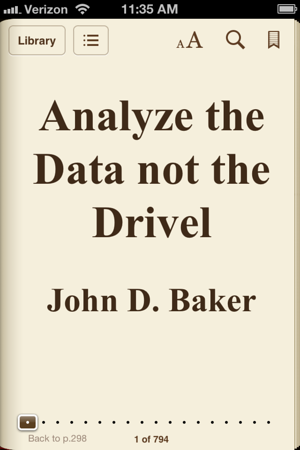
\includegraphics[width=0.50\textwidth]{i-BfnWMFz-M.png}
\caption{iPhone loaded with \href{http://www.box.com/s/ep9cgmdu6r3s322z5xim}{\texttt{bm.epub}}}
\label{fig:2587X0}
\end{minipage}
\hspace{1pt}
\begin{minipage}[b]{0.48\textwidth}
\centering
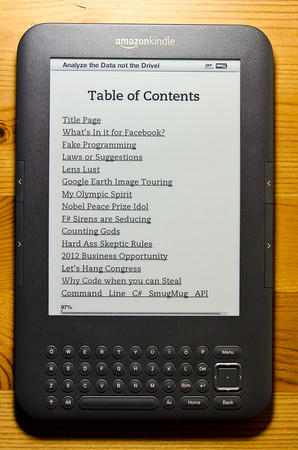
\includegraphics[width=0.50\textwidth]{i-dhqFDXQ-M.jpg}
\caption{Kindle loaded with \href{http://www.box.com/s/ttbyijqgmcnjzzsgfs0a}{\texttt{bm.mobi}}}
\label{fig:2587X1}
\end{minipage}
\end{figure}


%{[}caption id=``'' align=``aligncenter'' width=``162'' caption=``iPhone  loaded with my  blog''{]}
%\captionsetup[figure]{labelformat=empty}
%\begin{figure}[htbp]
%\centering
%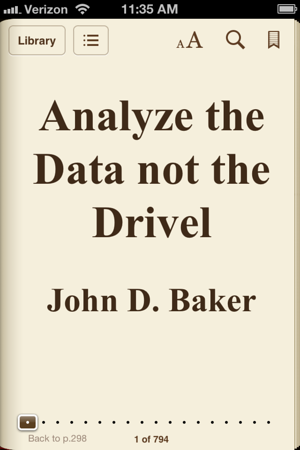
\includegraphics[width=0.23\textwidth]{i-BfnWMFz-M.png}
%\caption{iPhone  loaded with my  blog}
%\label{fig:2587X0}
%\end{figure}


The last step converts \texttt{bm.epub} to \href{http://www.box.com/s/ttbyijqgmcnjzzsgfs0a}{\texttt{bm.mobi}}. MOBI is a
native Kindle format. Pandoc can generate MOBI from \texttt{bm.markdown}
but it inexplicably omits a table of contents. \emph{No problemo:} I use
\href{http://calibre-ebook.com/}{Calibre} to convert \texttt{bm.epub} to
\texttt{bm.mobi}. Calibre properly converts the embedded EPUB table of
contents to MOBI. Here's \texttt{bm.mobi} on a Kindle.


%{[}caption id=``'' align=``aligncenter'' width=``179'' caption=``Kindle  loaded with my  blog''{]}
%\begin{figure}[htbp]
%\centering
%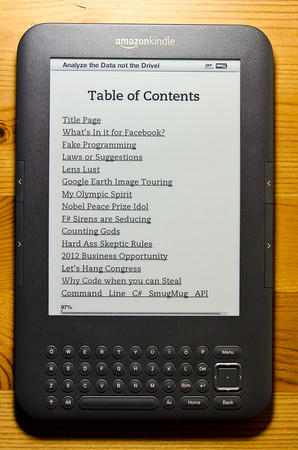
\includegraphics[width=0.23\textwidth]{i-dhqFDXQ-M.jpg}
%\caption{Kindle  loaded with my  blog}
%\label{fig:2587X1}
%\end{figure}


All the ``published'' versions of this blog are available on the
\textbf{\emph{\href{http://bakerjd99.wordpress.com/download-this-blog/}{Download
this Blog}}} page so please help yourself!


%\captionsetup[floatingfigure]{labelformat=empty}
%\begin{figure}[htbp]
%\begin{floatingfigure}[l]{0.25\textwidth}
%\centering
%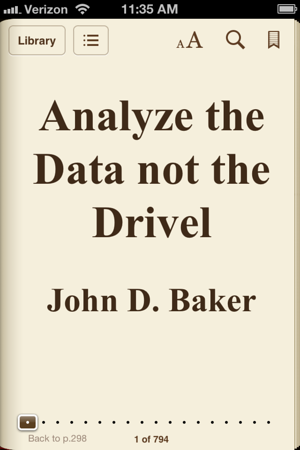
\includegraphics[width=0.23\textwidth]{i-BfnWMFz-M.png}
%\caption{~~~IMCAPTION~~~}
%\label{fig:2587X0}
%\end{floatingfigure}
%\end{figure}

%\captionsetup[floatingfigure]{labelformat=empty}
%\begin{figure}[htbp]
%\begin{floatingfigure}[l]{0.25\textwidth}
%\centering
%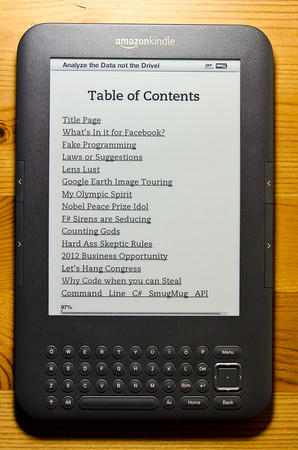
\includegraphics[width=0.23\textwidth]{i-dhqFDXQ-M.jpg}
%\caption{~~~IMCAPTION~~~}
%\label{fig:2587X1}
%\end{floatingfigure}
%\end{figure}



%\end{document}